\subsection{Anforderung}

Der Etikettendruckvorgang soll bei der Erstellung von Verkaufsbelegen, 
wie auch in der Lieferscheinauskunft ausgelöst werden. Als 
Anforderung ist die Schaffung eines Moduls zum Druck von Etiketten nach 
der \emph{GHS/CLP} Verordnung definiert. Das Etikett muss aussagekräftig
über den Hersteller (Name, Adresse, Telefon), der Menge des Stoffes oder 
Gemisches, der Produktidentifikation, der Gefahrenpiktogramme, der 
Signalwörter, der Gefahrenhinweise, der Sicherheitshinweise sowie über 
ergänzende Informationen sein. In Abbildung 
\ref{fig:musteretikett} ist ein solches Musteretikett sichtbar.

\begin{figure}[H]
    \centering
    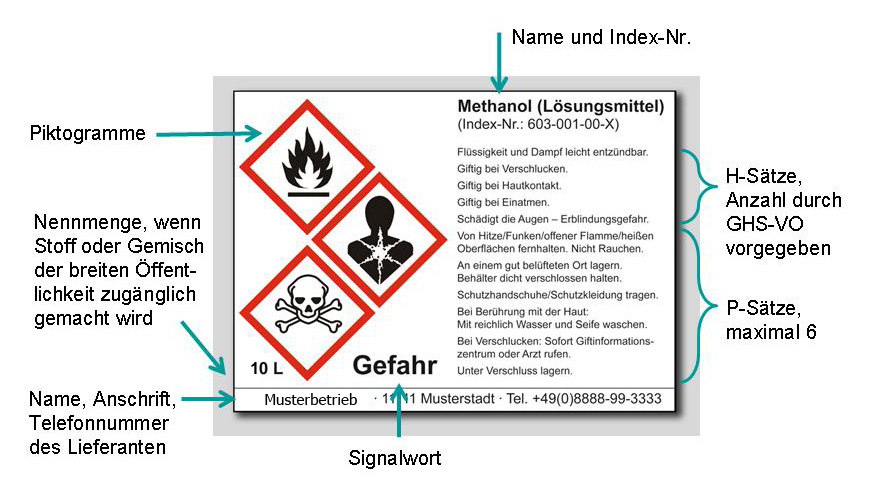
\includegraphics[height=200pt, width=320pt]{Beispieletikett.jpg}
    \caption[GHS Musteretikett]{\small{GHS Musteretikett. \cite{bgwetikett}}}
    \label{fig:musteretikett}
\end{figure}

\subsection{Ist-Zustand}

Gegenwärtig werden die Richtlinien nach der \emph{GHS/CLP} Verordnung für die 
Etiketten nicht von der Sage Office Line unterstützt. Aus diesem Grund werden 
bis zum Zeitpunkt der Moduleinführung die benötigten Etiketten, anhand einer PDF 
Vorlage, händisch von unserem Kunden erstellt. Die benötigten Daten hierfür 
kommen von einem Drittanbieter, welcher die Sicherheitsdatenblättern der 
jeweiligen Produkte erstellt. 

\noindent
Der derzeitige Ablauf der Etikettierung der Produkte erfolgt durch den 
Produktionsleiter. Dieser druckt anhand des Lieferscheins, 
direkt nach der Abfüllung des Produkts, das jeweilige händisch erstellte
Etikett mit der passenden Zweitsprache aus und klebt es auf die entsprechenden
Gebinde. Ein Gebinde ist eine Handelseinheit, welches Produkte gleicher Art bzw.
verschiedener Abfüllmengen zusammenfasst.\cite{gebinde} 
Bei der Abfüllung von Produkten in Säcken ist eine zusätzliche Etikettierung nicht notwendig, 
da diese bereits mit den benötigten \emph{GHS/CLP} Merkmalen bedruckt sind. \cite{fzp}

\begin{figure}[H]
    \centering
    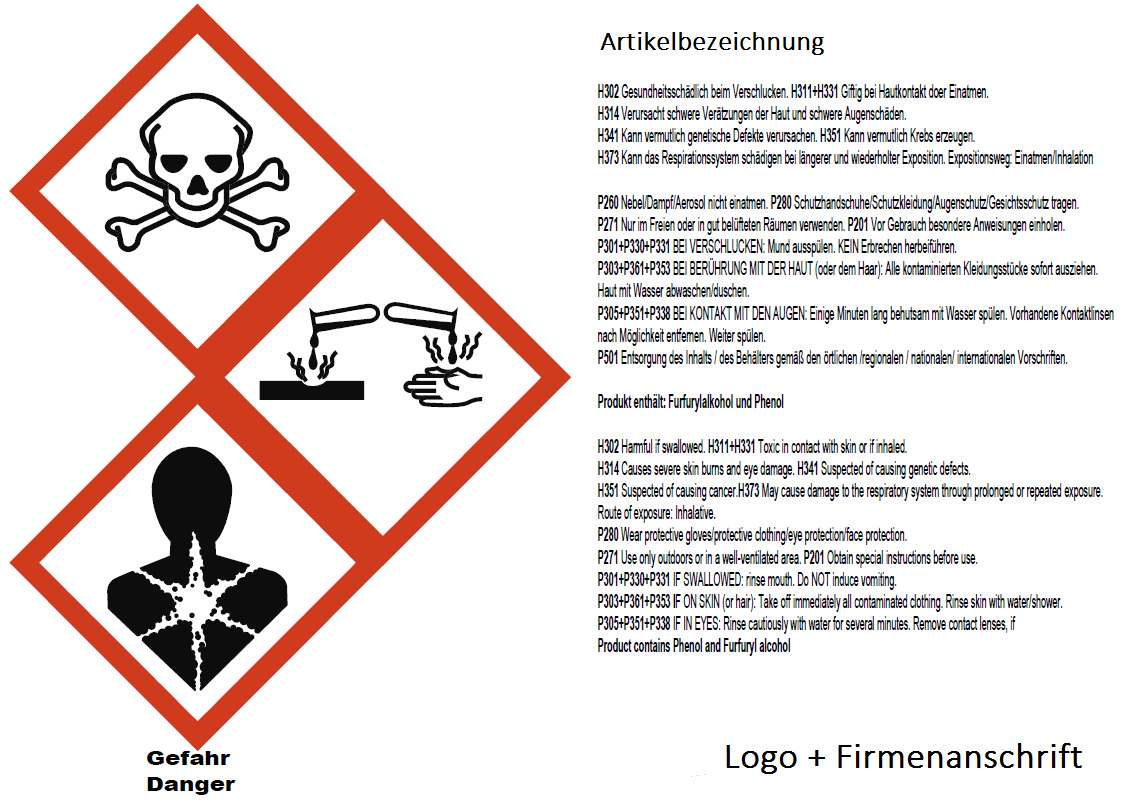
\includegraphics[height=280pt, width=400pt]{etikett_mod.png}
    \caption[händisch erstelltes Musteretikett]{\small{händisch erstelltes Musteretikett. \cite{fzp}}}
    \label{fig:hemusteretikett}
\end{figure}

\begin{figure}[H]
    \centering
    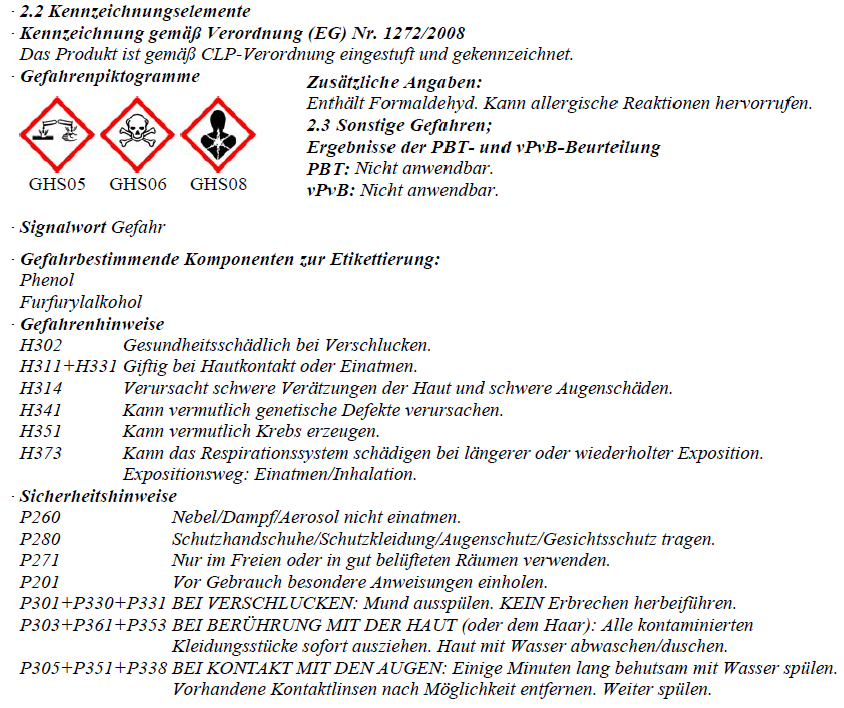
\includegraphics[height=285pt, width=330pt]{Sicherheitsdatenblatt.png}
    \caption[Muster Sicherheitsdatenblatt]{\small{Muster Sicherheitsdatenblatt. \cite{fzp}}}
    \label{fig:sicherheitsdatenblatt}
\end{figure}

\subsection{Ziele}
Das Hauptziel der Modulentwicklung ist die Abbildung der neuen gesetzlichen Voraussetzungen für 
Etiketten nach \emph{GHS/CLP} Verordnung in der Sage Office Line. Der Wechsel vom bestehenden,
manuellen Verfahren bis zur automatisierten Etikettenerzeugung ist ein weiteres Ziel. Daraus 
sollten zusätzliche Vorteile / Ziele resultieren, wie die Entlastung von Mitarbeitern, 
die Steigerung der Effizienz und die Reduzierung von Kosten.

\subsection{Planung}

Die Umsetzung des Projekts erfolgt in 2 Abschnitten. Im ersten Schritt 
ist es notwendig die Etiketten nach \emph{GHS/CLP} Verordnung 
zu erstellen und die Einbindung in die Sage Office Line zu realisieren. 
Der zweite Schritt umfasst die Programmierung des Etikettendesigners. Für die Entwicklung
des 1. Abschnitts war der Zeitraum von der 15. bis 19. Kalenderwoche sowie für den 2. Abschnitt 
der Zeitraum von der 20. bis 23. Kalenderwoche vorgesehen.

\subsubsection{Umstellung der Artikel}

Für eine bessere Zuordnung der Artikel zu den Etiketten wäre es vorteilhaft, 
gebindespezifische Artikel anzulegen. Dieser Schritt ist sinnvoll, da die 
Größe der Etiketten von der Füllmenge des Produktes abhängig ist. Jedoch ist 
dies ein größerer Eingriff in den aktuellen Unternehmensablauf und wird hier
nicht weiter berücksichtigt. Der Lösungsansatz um keine Prozesse ändern zu
müssen, ist der Aufruf einer Druckmaske nach dem Druck von Verkaufsbelgen 
oder Lieferscheinen. Mittels der Druckmaske lassen sich die Anzahl, wie auch 
die Größe der Etiketten nach \emph{GHS/CLP} Verordung für jeden Artikel
auswählen und drucken.

\begin{figure}[H]
    \centering
    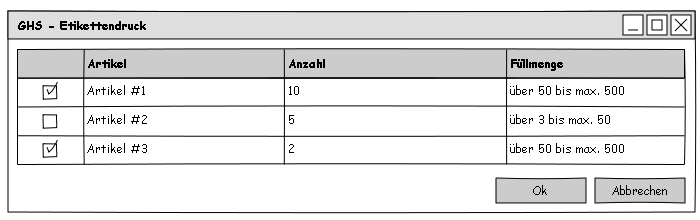
\includegraphics[height=130pt, width=\textwidth]{Druckmaske_2.png}
    \caption[Prototyp der Druckmaske]{\small{Prototyp der Druckmaske. \cite{fzp}}}
    \label{fig:prototypdruckmaske}
\end{figure}

\subsubsection{Erweiterung der Artikelstammdaten}
\label{subsubsec:erweiterungartikelstamm}

Zur Erstellung von Etiketten nach \emph{GHS/CLP} Verordnung ist es unabwendbar den 
Artikelstamm um die Eigenschaft „P-Sätze“ zu erweitern. Des Weiteren ist es 
erforderlich die Zweitsprache anhand der Adresse des Produktempfängers zu ermitteln. 
Die Auswahl der notwendigen Bestandteile der Etiketten erfolgt über fest 
definierte Auswahlfelder. Die Identifikationsnummern und Sprachpakete der 
offiziellen europäischen Amtssprachen stammen direkt von der Europäischen Union 
und werden mittels MS SQL\footnote{\label{foot:mssql}MS SQL: Die Abkürzung steht 
für Microsoft Structured Query Language und ist eine, von Microsoft entwickelte, 
Datenbanksprache für relationale Datenbanken "'zum Bearbeiten (Einfügen, Verändern, 
Löschen) und Abfragen von darauf basierenden Datenbeständen"'\cite{mssql}.}
– Skript bei Auslieferung des Moduls in die bestehende 
Datenbank integriert. Der Bezug der weiteren benötigten Sprachpakete für 
Arabisch (Ägyptisch), Chinesisch und Türkisch ist abschließend noch nicht 
geklärt. Es stehen diverse Online – Quellen von unterschiedlichen Anbietern zur Verfügung.
Die nachfolgende Abbildung zeigt die Erfassung der Arikelstammdaten vor der
geplanten Änderung.

\begin{figure}[H]
    \centering
    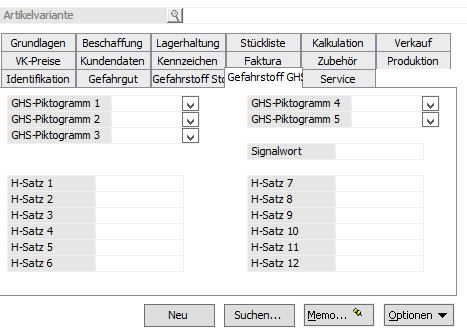
\includegraphics[height=230pt, width=320pt]{Artikelstamm.PNG}
    \caption[Arikelstammdatenerfassung]{\small{Arikelstammdatenerfassung. \cite{fzp}}}
    \label{fig:arikelstammdatenerfassung}
\end{figure}

\noindent
Die Abbildung \ref{fig:prototyparikelstammdatenerfassung} zeigt das geänderte Layout 
zur Erfassung der Artikelstammdaten anhand des Sicherheitsdatenblattes. Damit die 
Erfassung dynamisch gehalten werden kann, entfällt der Reiter \emph{Gefahrstoff GHS} 
im Artikelstamm (siehe Abbildung \ref{fig:arikelstammdatenerfassung}).

\begin{figure}[H]
    \centering
    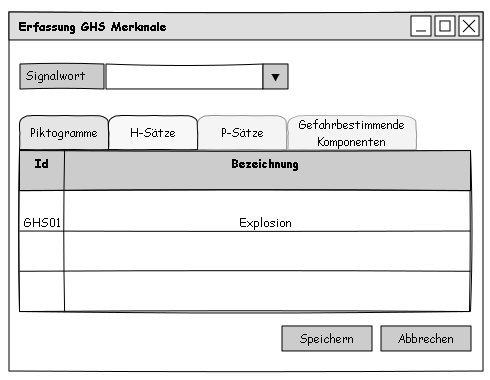
\includegraphics[height=170pt, width=330pt]{Stammdaten_3.png}
    \caption[Prototyp der Arikelstammdatenerfassung]
    {\small{Prototyp der Arikelstammdatenerfassung. \cite{fzp}}}
    \label{fig:prototyparikelstammdatenerfassung}
\end{figure}

\noindent
Die neue Erfassungsmaske kann über das Optionenmenü mittels dem Menüpunkt
\emph{GHS-Merkmale} ausgewählt werden. Weiterhin kann über den Menüpunkt
\emph{GHS-Etikettendesigner} der Etikettendesigner gestartet werden (siehe 
Abbildung \ref{fig:openerfassungsmaske1}).

\begin{figure}[H]
    \centering
    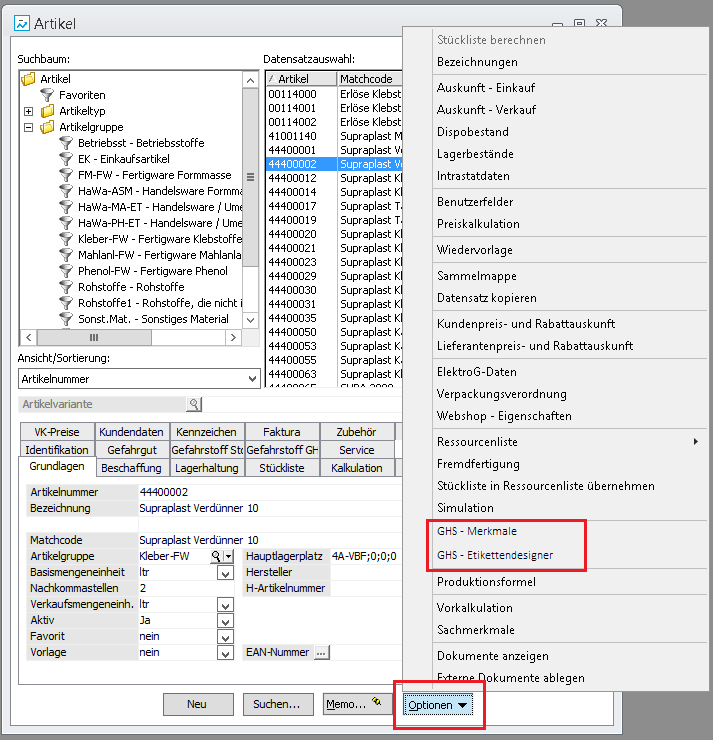
\includegraphics[height=360pt, width=430pt]{artikel_optionen_1.PNG}
    \caption[Öffnung Erfassungsmaske - Variante 1]
    {\small{Öffnung Erfassungsmaske - Variante 1. \cite{fzp}}}
    \label{fig:openerfassungsmaske1}
\end{figure}

\noindent
Außerdem können, wie in Abbildung \ref{fig:openerfassungsmaske2} zu sehen ist, 
über das Menü \emph{Extras | Schaltflächen} aus dem Optionsmenü 
Schaltflächen erzeugt werden, welche die Erfassungsmaske für die \emph{GHS/CLP} 
Merkmale sowie den Etikettendesigner direkt aufrufen können (GHS / Designer).

\begin{figure}[H]
    \centering
    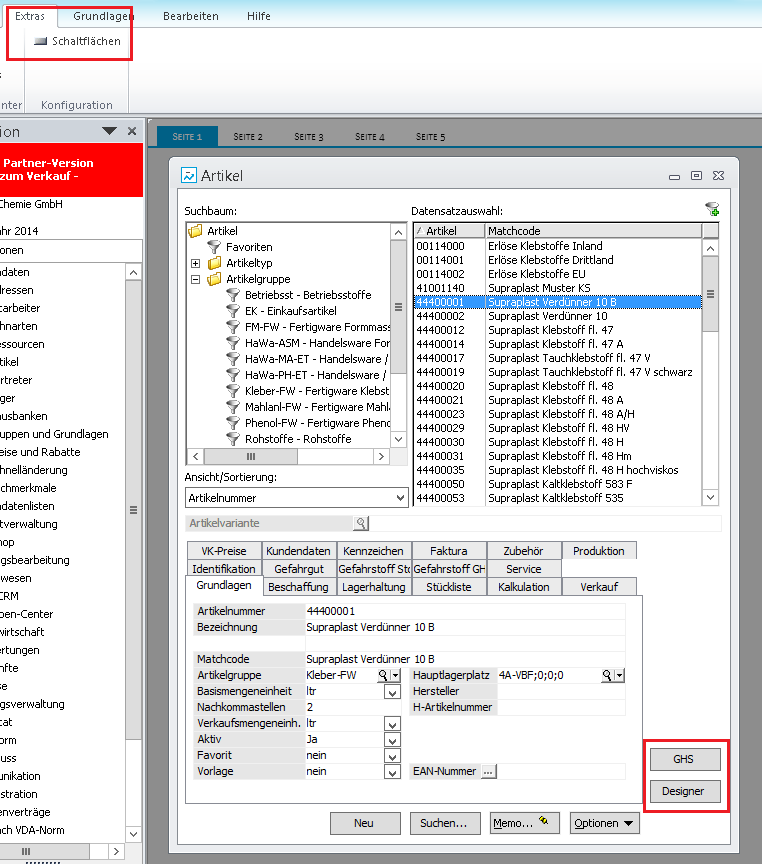
\includegraphics[height=410pt, width=430pt]{artikel_optionen_2.PNG}
    \caption[Öffnung Erfassungsmaske - Variante 2]
    {\small{Öffnung Erfassungsmaske - Variante 2. \cite{fzp}}}
    \label{fig:openerfassungsmaske2}
\end{figure}

\subsubsection{Erstellung der Etiketten}
\label{subsubsec:erstellungetiketten}
Zur Erstellung der Etiketten wird, anhand der gesetzlichen Vorgaben, eine selbst programmierte 
Vorlage verwendet. Hierbei ist zu beachten, dass die Größe der Etiketten sowie der Piktogramme 
an die Füllmenge des Produkts gekoppelt ist. Es müssen folgende Mindestabmessungen berücksichtigt 
werden:

\begin{table}[H]
\begin{tabular}{|l|l|l|}\hline
 \textbf{Füllmenge} & \textbf{Abmessung Etikett} & \textbf{Abmessung Piktogramm} \\
 \textbf{in l} & \textbf{in mm} & \textbf{in mm} \\ \hline
 bis 3 & wenn möglich min. 52 x 74 & min. 10 x 10, \\ & & wenn möglich 16 x 16 \\ \hline
 über 3 bis max. 50 & min. 74 x 105 & min. 23 x 23 \\ \hline
 über 50 bis max. 500 & min. 105 x 148 & min. 32 x 32 \\ \hline
 größer 500 & min 148 x 210 & min. 46 x 46 \\ \hline
\end{tabular}
\end{table}

\noindent
Die Etiketten sollen wie Folgt für die verschiedenen Piktogramm - Anzahlen aussehen:

\begin{figure}[H]
    \centering
    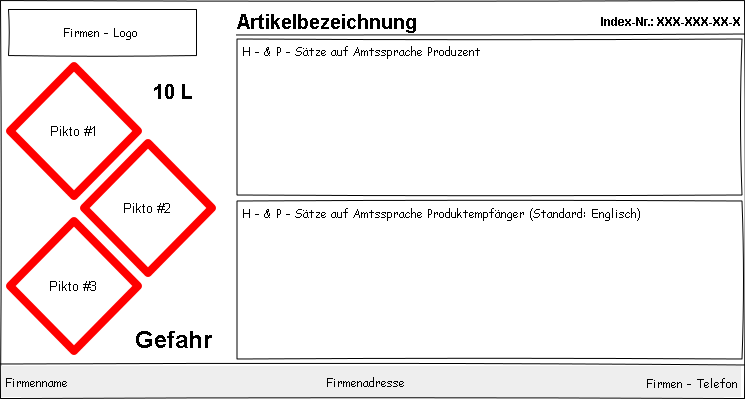
\includegraphics[height=170pt, width=340pt]{Musteretikett-3Pikto.png}
    \caption[Prototyp des Musteretiketts mit 3 Gefahrenpiktogramme]
    {\small{Prototyp des Musteretiketts mit 3 Gefahrenpiktogramme. \cite{fzp}}}
    \label{fig:prototypmusteretikett3p}
\end{figure}

\begin{figure}[H]
    \centering
    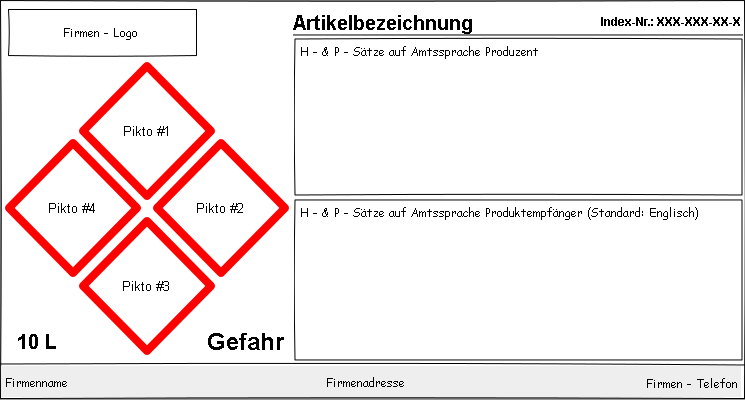
\includegraphics[height=170pt, width=340pt]{Musteretikett-4Pikto.png}
    \caption[Prototyp des Musteretiketts mit 4 Gefahrenpiktogramme]
    {\small{Prototyp des Musteretiketts mit 4 Gefahrenpiktogramme. \cite{fzp}}}
    \label{fig:prototypmusteretikett4p}
\end{figure}

\begin{figure}[H]
    \centering
    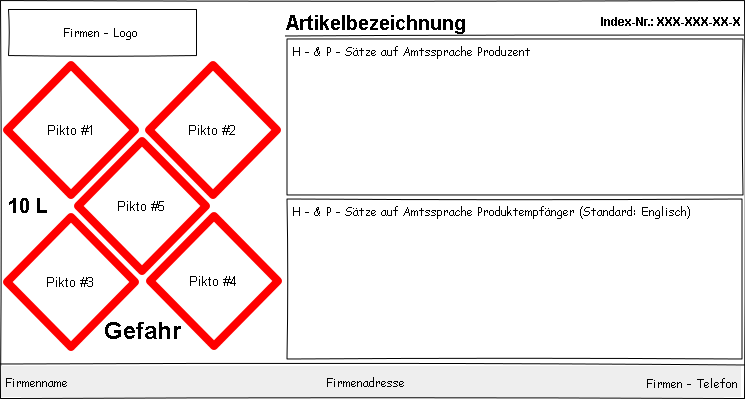
\includegraphics[height=170pt, width=340pt]{Musteretikett-5Pikto.png}
    \caption[Prototyp des Musteretiketts mit 5 Gefahrenpiktogramme]
    {\small{Prototyp des Musteretiketts mit 5 Gefahrenpiktogramme. \cite{fzp}}}
    \label{fig:prototypmusteretikett5p}
\end{figure}

\subsubsection{Erstellung des Etikettendesigner}
Mit dem Designer soll es möglich sein, Etiketten individuell gestalten zu können. 
Wichtig hierbei ist, dass bei selbsterstellten Etiketten die Prüfung der benötigten 
Etikettenbestandteile nach \emph{GHS/CLP} Verordnung vom Ersteller selbst 
durchgeführt werden muss. Der Designer soll ebenfalls, wie in Abbildung 
\ref{fig:openerfassungsmaske1} und \ref{fig:openerfassungsmaske2}
gezeigt, am Artikelstamm über das Optionsmenü aufgerufen werden können. 

\begin{figure}[H]
    \centering
    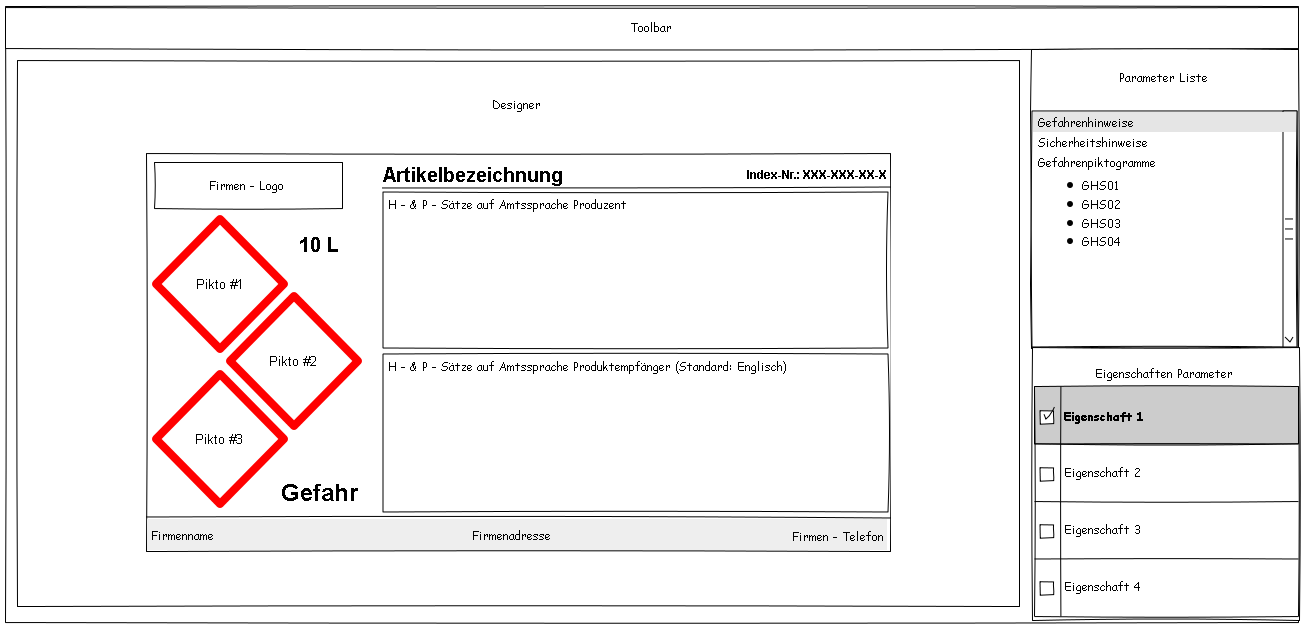
\includegraphics[height=240pt, width=\textwidth]{Etikettendesigner_1.png}
    \caption[Prototyp des Etikettendesigner]
    {\small{Prototyp des Etikettendesigner. \cite{fzp}}}
    \label{fig:prototypetikettendesigner}
\end{figure}